% Centri — Cases & Evaluation (focused deck)
% Compile: pdflatex -interaction=nonstopmode centri-cases-eval.tex   (run twice)
\documentclass[aspectratio=169,10pt]{beamer}
\usetheme{metropolis}
\metroset{sectionpage=progressbar, subsectionpage=none, numbering=fraction, progressbar=frametitle}

\usepackage{booktabs}
\usepackage{amsmath,amssymb}
\usepackage{siunitx}
\usepackage{xcolor}
\usepackage{colortbl}
\usepackage{graphicx}
\graphicspath{{figs/}}
\usepackage{tikz}
\usetikzlibrary{arrows.meta,positioning,calc,shapes.geometric,fit,backgrounds}
\usepackage[most]{tcolorbox}

% ---- palette -------------------------------------------------------------
\definecolor{cMeas}{HTML}{1F6FB2}
\definecolor{cPed}{HTML}{B5651D}
\definecolor{cApp}{HTML}{2E7D32}
\definecolor{cInfra}{HTML}{5E35B1}
\definecolor{cAccent}{HTML}{C62828}
\definecolor{cGrey}{HTML}{616161}
\definecolor{cBg}{HTML}{F4F6F8}
\setbeamercolor{frametitle}{bg=cMeas}
\setbeamercolor{progress bar}{fg=cAccent}

\setlength{\fboxrule}{0.8pt}
\newcommand{\bignum}[2]{%
  \fcolorbox{cMeas}{cMeas!10}{\parbox[t]{25mm}{\centering
    {\bfseries\large\color{cMeas} #1}\\[1pt]{\scriptsize #2}\strut}}}
\newcommand{\hl}[1]{{\bfseries\color{cAccent}#1}}

\tikzset{
  box/.style={rounded corners=2pt, draw=#1, line width=0.8pt, fill=#1!8,
              text=black, align=center, font=\scriptsize, inner sep=4pt, minimum height=7mm},
  node distance=6mm and 9mm,
  flow/.style={-{Stealth[length=2.2mm]}, line width=0.7pt, draw=cGrey},
  hot/.style={-{Stealth[length=2.6mm]}, line width=1.0pt, draw=cAccent},
  lbl/.style={font=\tiny\itshape, text=cGrey, fill=white, inner sep=1pt},
}

\title{Centri --- Cases \& Evaluation}
\subtitle{Measuring circular motion across real scenes, and how the material is evaluated}
\author{Damar Albaribin \quad\small (evaluation collaborator: Vinsa Kharisma)}
\institute{MSc Thesis --- advisor: Prof.\ Wu-Yuin Hwang}
\date{\today}

\begin{document}
\maketitle

% =========================================================================
\begin{frame}{What this talk covers}
\small
Two halves, both grounded in real captures:
\begin{itemize}\setlength\itemsep{3pt}
  \item \textbf{\color{cMeas}The cases} --- four real scenes spanning the three motion regimes
  (uniform, decelerating, accelerating, and a two-phase spin-up\,/\,coast-down), including a
  \hl{new} ceiling-fan recapture that exposed --- and fixed --- a measurement bug.
  \item \textbf{\color{cPed}The evaluation} --- how the generated learning material is scored:
  relevance against an authentic textbook reference, made into a real reference \emph{set}, plus a
  \hl{multimodal} score that brings the figure into the metric.
\end{itemize}
\vspace{0.4em}
{\footnotesize Every number on the following slides comes from tracking a real video frame by frame ---
no simulated data. Absolute scale on the new fan is provisional (one unmeasured length); all the
\emph{relative} kinematics ($\omega$, period, regime) are scale-free.}
\end{frame}

% =========================================================================
\section{The cases --- measurement across real scenes}

\begin{frame}{Four cases at a glance --- the three motion regimes}
\small
\begin{center}
{\footnotesize
\begin{tabular}{lllc}
\toprule
\textbf{Scene} & \textbf{Regime} & \textbf{Key kinematics} & \textbf{Coverage} \\
\midrule
Bicycle wheel        & uniform              & $\omega\!\approx\!$\hl{5.1}\,rad/s, $T\,$\hl{1.18}\,s, $a_c\,1.9$--$2.1$ & 93.8\% \\
Turntable            & decelerating         & hand-spun coast-down, $\alpha\!<\!0$                       & 100\% \\
Ceiling fan (toy)    & accelerating         & spin-up $\alpha=$\hl{1.18}\,rad/s$^2$, $a_c\,$\hl{21.8}, $r\,0.45$\,m & 100\% \\
\rowcolor{cMeas!8}
Ceiling fan (marker) & \textbf{two-phase}   & spin-up\,$\to$\,peak $\omega\,$\hl{3.5}\,$\to$\,coast, $a_c^{\max}\,7.4$ & 100\%$^\dagger$ \\
\bottomrule
\end{tabular}}
\end{center}
\vspace{0.5em}
{\scriptsize Each regime lets the material teach something different --- a steady wheel can't teach
angular \emph{acceleration}; the spin-up and the two-phase fan can. $^\dagger$The new fan's coverage is
from frequency mode (blade-pass), after the per-frame tracker failed --- next slides.}
\end{frame}

% ---- new fan: the measurement story ----
\begin{frame}{The new ceiling fan --- a measurement bug, caught and fixed}
\scriptsize
\begin{columns}[T]
\column{0.41\textwidth}
\centering
\includegraphics[height=0.80\textheight,keepaspectratio]{newfan_orbit_compare}
\column{0.59\textwidth}
\textbf{The recapture:} a 5-blade ceiling fan, \hl{orange paper marker} on one blade tip, 75\,s at
60\,fps --- it \emph{spins up then coasts down} (two-phase).
\vspace{0.4em}

\textbf{\color{cAccent}What went wrong (object / SAM3 mode):}
\begin{itemize}\setlength\itemsep{1pt}
  \item the auto-ROI collapsed onto a tiny \hl{232\,px} box on the \emph{hub} (magenta) ---
  it tracked a hub feature, not the marked blade
  \item it measured a \hl{60\,px} ``orbit'' (red) and mis-scaled it as 0.32\,m; the marker
  (blade tip, \hl{357\,px}, orange) was never tracked
  \item that hub feature read \emph{blade-passes}, inflating $\omega$ by $\sim$\hl{3.5$\times$}
\end{itemize}
\vspace{0.3em}
\textbf{\color{cApp}The fix:}
\begin{itemize}\setlength\itemsep{1pt}
  \item \textbf{colour mode} (local, \hl{20\,s} vs 50\,min) locks the orange marker $\to$ the
  \emph{correct} 357\,px blade-tip orbit
  \item \textbf{frequency mode} (blade-pass FFT) recovers the true two-phase $\omega(t)$
\end{itemize}
\vspace{0.3em}
{\scriptsize \textbf{Lesson:} 100\% coverage and a clean-looking circle are \emph{not} enough ---
the orbit has to be the \emph{right} one. Identical blades + an auto-ROI is exactly the trap the
extra tracking modes exist for.}
\end{columns}
\end{frame}

\begin{frame}{The new fan --- three independent measurements agree}
\scriptsize
The corrected reading: a clean \textbf{two-phase} profile --- spin-up to a peak of $\omega\!\approx\!$\hl{3.5}\,rad/s
at $t\!\approx\!15$\,s, then a coast-down. Three independent methods converge:
\vspace{0.2em}
\begin{columns}[T]
\column{0.62\textwidth}
\includegraphics[width=\linewidth]{newfan_omega_validation}
\column{0.38\textwidth}
\begin{itemize}\setlength\itemsep{3pt}
  \item \textbf{\color{cMeas}frequency} (blade-pass FFT) --- blur-immune, the full $\omega(t)$
  \item \textbf{\color{cPed}colour marker} --- the real blade tip, where the marker is visible
  \item \textbf{\color{cApp}object\,$\div3.5$} --- the hub feature, de-inflated
\end{itemize}
\vspace{0.4em}
{\scriptsize Result (provisional 0.6\,m orbit): mean $a_c\,$\hl{2.3}, peak $a_c\,$\hl{7.4}\,m/s$^2$;
$T\,4.2$\,s. \emph{Relative} kinematics are exact; the metre-scale is one unmeasured length away.}
\end{columns}
\vspace{0.2em}
{\scriptsize \textbf{Honest caveat:} the single-regime classifier labels the clip ``accelerating''
(it fits one $\alpha$); the faithful two-phase $\omega(t)$ is kept in the measurement record. Extending
the classifier to two-phase motion is on the roadmap.}
\end{frame}

% =========================================================================
\section{Evaluation --- how the material is scored}

\begin{frame}{Material relevance --- the reference set and the score}
\scriptsize
BERTScore vs authentic OpenStax \S6.2, reorganized into our 5-section format --- each of the \hl{9}
prose sources scored per source (mean\,$\pm$\,SD across the \hl{5} runs). Numbers are ours; the metric
is the prior method's.
\vspace{0.2em}
\begin{columns}[T]
\column{0.53\textwidth}
{\tiny
\begin{tabular}{llc}
\toprule
\textbf{Source (the reference set)} & \textbf{Type} & \textbf{F1 (M\,$\pm$\,SD)} \\
\midrule
OpenStax \S6.2 (gold)              & textbook    & \hl{0.840}\,$\pm$\,0.002 \\
Edexcel / Physics\,\&\,Maths Tutor & revision    & 0.837\,$\pm$\,0.004 \\
Flipping Physics --- intro         & notes       & 0.834\,$\pm$\,0.003 \\
MIT OCW 8.01 Ch.6                  & chapter     & 0.828\,$\pm$\,0.003 \\
arXiv 1602.06361                  & paper       & 0.824\,$\pm$\,0.002 \\
EMU PHYS101                       & notes       & 0.824\,$\pm$\,0.003 \\
Univ.\ Alabama PH101               & notes       & 0.824\,$\pm$\,0.002 \\
USNA / Mungan                     & derivation  & 0.820\,$\pm$\,0.003 \\
Flipping Physics --- deriv         & derivation  & 0.814\,$\pm$\,0.004 \\
\midrule
\textbf{set mean}                 &             & \hl{0.827}\,$\pm$\,0.008 \\
\bottomrule
\end{tabular}}
\column{0.47\textwidth}
{\footnotesize\textbf{Does it depend on one reference? --- two results}}\\[2pt]
{\footnotesize
\begin{tabular}{lcc}
\toprule
\textbf{Prose set} & \textbf{reorganized} & \textbf{raw} \\
\midrule
set mean & \hl{0.827} & 0.801 \\
SD       & 0.008      & 0.012 \\
\bottomrule
\end{tabular}}\\[3pt]
{\scriptsize Reorganizing each reference into our format lifts \emph{and} tightens the score
(\hl{+0.026}; all 9 improve). Per-section peaks on \emph{``how the variables relate''} (\hl{0.852}),
dips on the grounded sections --- our value-add the textbook lacks.}\\[3pt]
\begin{tcolorbox}[colback=cMeas!5,colframe=cMeas!45,boxrule=0.3pt,left=3pt,right=3pt,top=2pt,bottom=2pt]
{\tiny\textbf{Example (OpenStax \S6.2, ``how the variables relate'', as reorganized):} ``For an object
in a circle of radius $r$ at speed $v$, $a_c=v^2/r$\,\dots\ it points toward the centre.''}
\end{tcolorbox}
\end{columns}
\vspace{0.2em}
{\scriptsize BLEU / ROUGE planned.}
\end{frame}

\begin{frame}{The reference set --- diagnostic buckets (10 sources, raw)}
\scriptsize
The remaining \hl{10} sources are \emph{not} five-section learning material --- lecture slides,
worksheets, lab sheets. Reported \emph{separately} (raw, mean\,$\pm$\,SD), as diagnostics, not the gold.
\vspace{0.2em}
\begin{columns}[T]
\column{0.6\textwidth}
{\tiny
\begin{tabular}{llc}
\toprule
\textbf{Source} & \textbf{Bucket} & \textbf{F1 (M\,$\pm$\,SD)} \\
\midrule
Univ.\ Hawaii P170       & slides    & 0.823\,$\pm$\,0.003 \\
Ohio State P111          & slides    & 0.819\,$\pm$\,0.002 \\
Univ.\ Sydney Mech.\ L6   & slides    & 0.813\,$\pm$\,0.002 \\
UIUC P101 handout        & slides    & 0.807\,$\pm$\,0.001 \\
\midrule
USC UCM lab (PHYS 201)   & lab       & 0.824\,$\pm$\,0.005 \\
Univ.\ Oklahoma L8        & lab       & 0.815\,$\pm$\,0.005 \\
\midrule
APlusPhysics UCM         & worksheet & 0.815\,$\pm$\,0.003 \\
Colorado Mesa Handout 18 & worksheet & 0.810\,$\pm$\,0.002 \\
Boston Univ.\ UCM         & worksheet & 0.796\,$\pm$\,0.003 \\
UBC concept questions    & worksheet & 0.782\,$\pm$\,0.002 \\
\bottomrule
\end{tabular}}
\column{0.4\textwidth}
{\tiny\textbf{Bucket means:}}\\[2pt]
{\tiny
\begin{tabular}{lc}
\toprule
\textbf{Bucket} & \textbf{F1 (M\,$\pm$\,SD)} \\
\midrule
lab instructions & 0.820\,$\pm$\,0.007 \\
lecture slides   & 0.815\,$\pm$\,0.006 \\
worksheets / Q   & 0.801\,$\pm$\,0.013 \\
\bottomrule
\end{tabular}}\\[4pt]
{\tiny These describe problems and figures, not five-section material --- a robustness band, not
the gold. The raw sources vary in scope, so SDs run wider (esp.\ worksheets). OpenStax \S6.2 is
uniform-motion only --- more non-uniform references to add.}
\end{columns}
\end{frame}

\begin{frame}{Multimodal relevance --- bringing the \emph{figure} into the metric}
\small
BERTScore is a text metric, so a generated \emph{figure} never enters it. We let a vision model
\hl{caption} each figure (image\,$\to$\,text), then BERTScore the caption against the reference
\emph{figure}'s caption (OpenStax \S6.2's own diagrams). The image input now flows through the
\emph{same} metric as the prose.
\vspace{0.3em}
\begin{columns}[T]
\column{0.44\textwidth}
\centering
{\footnotesize
\begin{tabular}{lccc}
\toprule
\textbf{Stat} & \textbf{P} & \textbf{R} & \textbf{F1} \\
\midrule
M  & 0.832 & 0.827 & \hl{0.829} \\
SD & 0.005 & 0.002 & 0.004 \\
\bottomrule
\end{tabular}}\\[3pt]
{\scriptsize Visual channel \hl{0.829}\,$\pm$\,0.004, beside the prose channel 0.840.}\\[6pt]
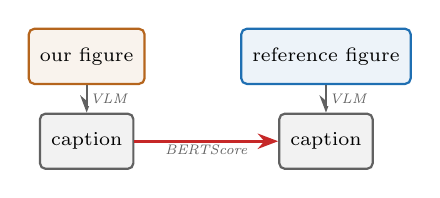
\begin{tikzpicture}[font=\scriptsize,node distance=3.5mm]
  \node[box=cPed] (f) {our figure};
  \node[box=cMeas, right=12mm of f] (rf) {reference figure};
  \node[box=cGrey, below=of f] (c) {caption};
  \node[box=cGrey, below=of rf] (rc) {caption};
  \draw[flow] (f)--(c) node[lbl,midway,right]{VLM};
  \draw[flow] (rf)--(rc) node[lbl,midway,right]{VLM};
  \draw[hot] (c)--(rc) node[lbl,midway,below]{BERTScore};
\end{tikzpicture}
\column{0.56\textwidth}
{\tiny\textbf{Example --- the two captions that get scored:}}
\begin{tcolorbox}[colback=cPed!5,colframe=cPed!45,boxrule=0.3pt,left=3pt,right=3pt,top=2pt,bottom=2pt]
{\tiny\textbf{\color{cPed}our figure $\to$ VLM caption:} ``A ceiling fan with five blades, a yellow toy
on one blade; a green circle marks the rotation path about the hub --- radius $r=0.454$\,m, the
circular trajectory.''}
\end{tcolorbox}
\vspace{1pt}\centering{\tiny $\downarrow$ \textbf{BERTScore} $\uparrow$}\\[1pt]
\begin{tcolorbox}[colback=cMeas!5,colframe=cMeas!45,boxrule=0.3pt,left=3pt,right=3pt,top=2pt,bottom=2pt]
{\tiny\textbf{\color{cMeas}reference figure $\to$ VLM caption:} ``Two scenarios of circular motion:
a car on a curved road, and a centrifuge; radius $r$ from the centre, tangential velocity $v$,
centripetal acceleration $a_c$ pointing toward the centre.''}
\end{tcolorbox}
\vspace{2pt}
{\tiny Captions verified faithful --- they read our \emph{actual} values ($r=0.454$\,m), no
hallucination. Annotated frame + summary panel match this car\,/\,centrifuge figure strongest ($\approx$0.85).}
\end{columns}
\end{frame}

% =========================================================================
\begin{frame}{Summary}
\small
\begin{itemize}\setlength\itemsep{4pt}
  \item \textbf{Four real cases} span the motion regimes; the new ceiling fan added a genuine
  \hl{two-phase} capture --- and a caught-and-fixed measurement bug (hub ROI $\to$ colour\,+\,frequency).
  \item Measurement is \textbf{cross-checked}: three independent methods agree on the new fan's
  $\omega(t)$ (peak $\approx$\hl{3.5}\,rad/s).
  \item Material relevance is \hl{0.840} vs the gold textbook, \hl{0.827} across a reorganized
  reference \emph{set} --- not an artifact of one reference (raw \emph{0.801}; every reference
  improves with reorganization).
  \item References are \textbf{classified}; question/slide/lab sources are reported separately.
  \item A \textbf{multimodal} score (\hl{0.829}) brings the figure into the same metric.
\end{itemize}
\vspace{0.4em}
{\scriptsize Honest scope: absolute scale on the new fan is provisional; the two-phase classifier
and more non-uniform references are on the roadmap. Relative kinematics and the evaluation method
stand regardless.}
\end{frame}

\end{document}
